The PC environment had morphed significantly between the development of Wolfenstein 3D in 1991 and the development of Doom in 1993. The previous "recommend configuration" based on an Intel 386 CPU with 2~MiB of RAM and a VGA graphic card was no more.\\
\par
The "new" typical PC still had six subsystems \circled{1}~Inputs, \circled{2}~Bus, \circled{3}~CPU, \circled{4}~RAM, \circled{5}~Video~output, and \circled{6}~Audio~output together forming a pipeline. Only each of them had become faster or increased its capacity.\\
\par
\vspace{2mm}
\drawing{pc_components}{The six components of an IBM PC.}
\par
 Before describing each components in details, an important clarification is required. Since this chapter is structured as a delta comparing what was available for \doom to what was available for Wolfenstein 3D, it carries a feeling of abounding power which is deceiving. \\
 \par
 Despite the impressive list of improvements listed next, keep in mind that the IBM PCs were still not machines well suited for video games. They were riddled with limitations due to the original target which was office work. The goal was to perform word processing, write spreadsheet, accounting. Maybe sometimes display a static graph. The target was never to build something allowing real time, 70Hz\footnote{The VGA refresh rate was 70Hz contrary to today ubiquitous 60Hz.} animations.\\ 
\par 
Looking back it is almost hard to believe that some studios focused solely on producing titles for a machine seemingly less capable than consoles. The list of problems is substantial.
\begin{itemize}
\item A CPU unable to perform floating-point operations.
\item An archaic graphic system unable no double buffer and distorting images.
\item A sound system only capable of irritating "beeps" and a fragmented sound card ecosystem when the customer had elected to buy one.
\item A pricetag where a top of line machine fetched close to \$13,000 adjusted to inflation. To compare with competitions, the SNES and the SEGA Genernis were both priced at US\$199 while the Neo-Geo which provided arcade-like experience was US\$649.99.
\end{itemize}
\par
 A PC was unappealing at best and seemingly less likely to generate good games and profit, especially compared to cheaper systems such as the Super Nintendo, the Sega Genesis, or the NeoGeo systemswhich were designed from the ground up for video games. Obviously, given the title of the book you have in your hands, with a few software tricks the hardware of the PC was capable of far more than what it was designed for. PCs were not good at certain types of game (anything involving sprites) but they could excel at certain types of 3D engines.But keep in mine that on paper it was a challenge far from being trivial.\\
\par

In figure ~\ref{ibm_ps1_top}, an ad from 1994 for an IBM PS1 featuring an Intel 486 CPU with two things to notice.
\begin{itemize}
\item The emphasis office work and static screen office apps, the only way to justify the outrageous price of the machine (\$2,000\footnote{\$13,000 in 2017.}). 
\item The standard 14" CRT which probably weighted close to 20 pounds!\\
\end{itemize}
\par
\vspace{2 in}
\par
\begin{figure}[H] \centering
\fullimage{ibm_ps1_top}
\caption{IBM PS/1 ad circa 1994}
\label{ibm_ps1_top}
\end{figure}


















\cleartoleftpage
 
\cfullimage{PX486P3/b-486-px486p3_romain}{Motherboard PX486P3 by QDI Computer, Inc}
The best way to get an overview of the changes is to look at the component connecting them all together. The best selling motherboard of the year 1993 was the PX486P3 by QDI Computer, Inc\footnote{Again, a canadian company :) !}.\\

\par
The most prominent novelty is of course the heart of the computer, the Intel i486 CPU (\circled{1}). Yet a closer looks reveals many more features which would turn out to be of paramount importance for the architecture of \doom engine.\\
\par 
If the black extension connectors show the traditional ISA bus ports, one 8 bit (\circled{2}), three dual slot 16 bit (\circled{3}) we can also see a set of three new type of connector with an additional brown slot (\circled{4}). These are VL-Bus\footnote{Video Local Bus.}, a new type of bus up to 20x faster than ISA.

\drawing{px486p3}{Components diagram of the PX486P3.}
\par
 Next in the upper right (\circled{5}), a new type of RAM had found its way into these new PC. These eight black chips of Static RAM offered 256 KiB acting as "cache", a new system to prevent CPU starvation. SRAM\footnote{Static RAM} had an access time of 20ns, which was 10x faster than dRAM\footnote{Dynamic RAM}. It aimed at avoiding CPU stalls within the pipeline\footnote{SRAM was expensive and took a lot of space. SRAM was not only expensive, it also took a lot of space. Despite their size compared to the DRAM (in white), these eight chips could only stored 256 KiB with 20ns access time.}. \\
\par
The main memory system had grown in capacity, speed and complexity. Thanks to a sharp decline in manufacturing price, the standard DRAM installed (\circled{6}) had doubled to 4MiB\footnote{\doom would not run on PC equipped with "only" 2 MiB}.


\begin{center}
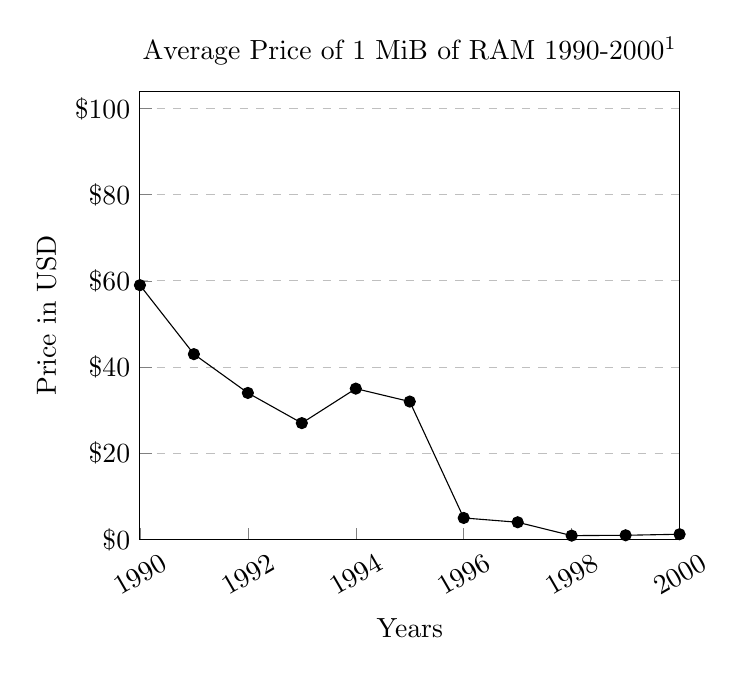
\begin{tikzpicture}

\begin{axis}[
    title={Average Price of 1 MiB of RAM 1990-2000\protect\footnotemark},
    xlabel={Years},
    xtick pos=left,
    ytick pos=left,
    ylabel={Price in USD},
    yticklabel={${\$\pgfmathprintnumber{\tick}}$},
    xticklabel style={ rotate=30,},
    xticklabel style={/pgf/number format/1000 sep=},
    xmin=1990, xmax=2000,
    ymin=0, ymax=104,
    %xtick={0,20,40,60,80,100},
    %ytick={0,20,40,60,80,100,120},
    legend pos=north west,
    ymajorgrids=true,
    grid style=dashed,
]
 
\addplot[
    color=black,
    mark=*,
    ]
    coordinates {
    (1990,59)
      (1991,43)
      (1992,34)
      (1993,27)
      (1994,35)
    (1995,32)
      (1996,5)
      (1997,4)
      (1998,0.9)
      (1999,0.98)
      (2000,1.22)
    
    };
 
\end{axis}
\end{tikzpicture}
\end{center}
\footnotetext{Source: John C. McCallum survey.}
% \begin{enumerate}
% \item RAM prices had dropped significantly. The standard 2 MiB was not a whooping 4 MiB. 
% \item Bandwidth hungry GUI and had lead motherboard manufacturers to come up with a faster bus called VLB.
% \item The sound generator ecosystems was even more fragmented than before with more and more manufacturer producing sound cards.
% \item Not visible on the drawing, the operating system shortcomings were being addressed by independent developers via something called "DOS eXtenders".
% \item Unsurprisingly the impossible to program VGA was still the standard but manufacturers were now competing to produce the faster DACs and \fixme{"RAMDAC"}?.
% \item CACHE
% \end{enumerate}
\par
\trivia{Several of the most impressive game studio of the era speculated on the projected price drop. Big titles of 1994 all required a minimum of 4 MiB installed. Strike Commander, Ultima 8, and Commanche Maximum Overkill are prime examples.

\begin{center}
\scaledimage{0.31}{box_strike_commander.png} \scaledimage{0.31}{box_ultima8.png} \scaledimage{0.31}{box_comanche.png}
\end{center}
}
Ironically this time period would end up coinciding with the great RAM shortage of 1994 which saw the price go back up. The legend attributes the surge to a resin factory burning in Taiwan. In all likelihood the fluctuation is due to the release of the new operating system by Microsoft, Windows 95 which recommended a machine with 8 MiB RAM.
\break





